\documentclass{beamer}

\usepackage{tikz}

\begin{document}

\begin{frame}
\frametitle{Labyrinthe de démonstration}
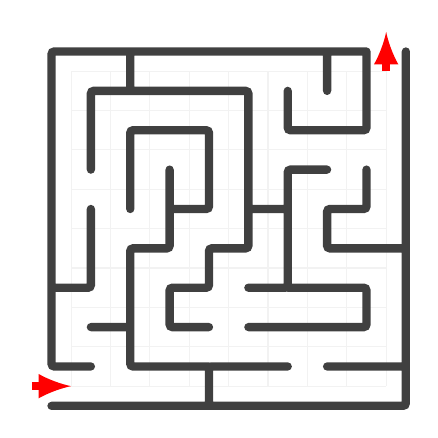
\begin{tikzpicture}[scale=.5]
  % Grid
  \draw[lightgray!20] (0,0) grid (8,8);
  
  % Puzzle
  \draw[line width=3pt,
  cap=round,
  rounded corners=1pt,
  draw=black!75] (-0.5,-0.5) -| (8.5,8.5)
  (7.5,8.5)-|(-0.5,0.5) -- (0.5,0.5) (-0.5,2.5)-|(0.5,4.5)
  (0.5,5.5)|-(4.5,7.5)|-(3.5,3.5)|-(2.5,2.5)|-(3.5,1.5)
  (8.5,0.5)--(6.5,0.5)
  (5.5,0.5)-|(3.5,-0.5)
  (3.5,0.5)-|(1.5,3.5)-|(2.5,5.5)
  (2.5,4.5)-|(3.5,6.5)-|(1.5,4.5)
  (7.5,8.5)|-(5.5,6.5)--(5.5,7.5)
  (6.5,7.5)--(6.5,8.5)
  (8.5,3.5)-|(6.5,4.5)-|(7.5,5.5)
  (6.5,5.5)-|(5.5,2.5)--(4.5,2.5)
  (5.5,2.5)-|(7.5,1.5)--(4.5,1.5)
  (5.5,4.5)--(4.5,4.5)
  (1.5,1.5)--(0.5,1.5)
  (1.5,7.5)--(1.5,8.5);
  
  % Start and End Points
  \onslide<2>{\draw[-latex,line width=3pt,red] (-1,0)--(0,0);}
  \onslide<3>{\draw[-latex,line width=3pt,red] (8,8) -- (8,9);}
\end{tikzpicture}
\end{frame}
\end{document}